\begin{figure}[!ht] 
    \centering
    \def\angle{0}
    \def\radius{3}
    \def\cyclelist{{"orange","blue","red","green","violet"}}
    \newcount\cyclecount \cyclecount=-1
    \newcount\ind \ind=-1
    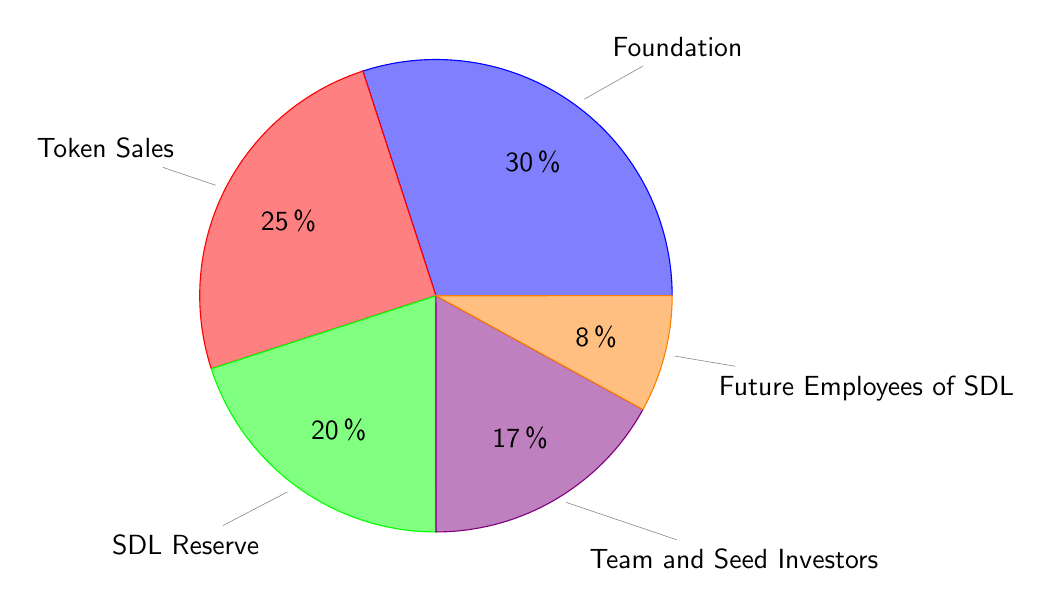
\begin{tikzpicture}[nodes = {font=\sffamily}]
    \foreach \percent/\name in {
          30/Foundation,
          25/Token Sales,
          20/SDL Reserve,
          17/Team and Seed Investors,
          8/Future Employees of SDL
        } {
          \ifx\percent\empty\else               % If \percent is empty, do nothing
            \global\advance\cyclecount by 1     % Advance cyclecount
            \global\advance\ind by 1            % Advance list index
            \ifnum4<\cyclecount                 % If cyclecount is larger than list
              \global\cyclecount=0              %   reset cyclecount and
              \global\ind=0                     %   reset list index
            \fi
            \pgfmathparse{\cyclelist[\the\ind]} % Get color from cycle list
            \edef\color{\pgfmathresult}         %   and store as \color
            % Draw angle and set labels
            \draw[fill={\color!50},draw={\color}] (0,0) -- (\angle:\radius)
              arc (\angle:\angle+\percent*3.6:\radius) -- cycle;
            \node at (\angle+0.5*\percent*3.6:0.7*\radius) {\percent\,\%};
            \node[pin=\angle+0.5*\percent*3.6:\name]
              at (\angle+0.5*\percent*3.6:\radius) {};
            \pgfmathparse{\angle+\percent*3.6}  % Advance angle
            \xdef\angle{\pgfmathresult}         %   and store in \angle
        \fi
        };
    \end{tikzpicture}
    \caption{Protocol token distribution breakdown. The total supply is capped at 13.5 billion.}
    \label{fig:TokenDistribution}
\end{figure}